\documentclass{article}
\usepackage[utf8]{inputenc}
\usepackage[T1]{fontenc}
\usepackage[a4paper, portrait, margin=1in]{geometry}
\usepackage{graphicx}
\usepackage{subcaption}
\usepackage{xcolor}
\usepackage{colortbl}
\usepackage{amscd,amsmath,amssymb,amsthm}
\usepackage{array}
\usepackage{mathtools}
\usepackage{bbm,dsfont}
\usepackage{lipsum}
\DeclareMathAlphabet{\mathbbold}{U}{bbold}{m}{n}
\parindent=15pt
\parskip=0pt plus 2pt

\newtheorem{theorem}{Theorem}

\newcommand{\0}{\mathbbold{0}}
\newcommand{\1}{\mathds{1}}
\newcommand{\diag}[1]{\text{diag}\!\left(#1\right)}
\newcommand{\Beta}[2]{\text{Beta}\!\left(#1,#2\right)}
\newcommand{\BBeta}[2]{\textbf{Beta}\!\left(#1,#2\right)}
\newcommand{\Lh}[2]{L\!\left(#1 \mid #2\right)}
\newcommand{\LRA}{\Leftrightarrow\mkern40mu}
\newcommand{\GEV}[3]{\text{GEV}\!\left(#1,#2,#3\right)}
\newcommand{\GEVcdf}[4]{\text{GEV}_\text{cdf}\!\left(#1;#2,#3,#4\right)}
\newcommand{\openinter}[2]{\left]#1,#2\right[}
\newcommand{\lopeninter}[2]{\left]#1,#2\right]}
\newcommand{\ropeninter}[2]{\left[#1,#2\right[}

\title{
\textbf{\huge{Development of an Intelligent Tutoring System using mixture modelling of learning curves}}
}
\author{\Large{\textsc{Tiago Quintas}}}
\date{\today}
\begin{document}
\maketitle
\begin{abstract}
    The web application SIACUA is a web plataform created to assist calculus students for an autonomous learning experience.
    To enhance the students' learning capabilites, over the years a new Intelligent Tutoring System (ITS) was being implemented, to provide guidance and recommendations to the user.
    In this paper we present an ITS capable of drawing learning curves and surfaces for each student individually and for the global dataset, while recommending various study tips in real time.
    Mixture modelling and bayesian inference were used to draw the learning curves and surfaces, as well as $t$-tests for the ITS's decision patterns, taking advantage of the bayesian networks already implemented in SIACUA.
\end{abstract}
\section{Introduction}
\begin{itemize}
    \item Why an ITS?
    \item How does SIACUA work?
    \item What are the ITS' objectives?
\end{itemize}
\subsection{Related Work}
\begin{itemize}
    \item What other papers have done?
\end{itemize}
\section{Mixture modelling}
Imagine a student starts answering a question of difficulty $i$, while having a knowledge belief of $b_1$ for that topic.
If we consider the binary set $e = \left\{0,1\right\}$ for the two outcomes for the answer, where $0$ means a correct answer and $1$ an incorrect answer,
we can represent the full action with a vector for the question, ${\bf q}_i$, a number for the belief, $b_1$, and a number for the answer, $e_1$.
\[ {\bf q}_i = [\underbrace{0 ~~ 0 ~~ \hdots \overbrace{1}^{i\textsuperscript{th}\text{ position}} \hdots ~~ 0}_d]^T \]
After answering a total of $n$ questions, we can construct a question matrix, ${\bf Q}$, a beliefs vector, ${\bf b}$, and an error vector, ${\bf e}$, such that
\begin{align*}
    {\bf Q} &= \begin{bmatrix}
        {\bf q}_1 & {\bf q}_2 & {\bf q}_3 & \hdots & {\bf q}_n
    \end{bmatrix}, ~~ {\bf Q} \in \mathcal{M}_{d\times n}\left(\left\{0,1\right\}\right) \\
    {\bf b} &= \begin{bmatrix}
        b_1 & b_2 & b_3 & \hdots & b_n
    \end{bmatrix}^T, ~~ {\bf b} \in \mathcal{M}_{n\times 1}\left([0,1]\right) \\
    {\bf e} &\in \left\{0,1\right\}^n.
\end{align*}
The matrix ${\bf Q}$ is called in this paper a \textsl{XOR Matrix by columns}, meaning that ${\bf Q}^T \cdot \1_d = \1_n$, where
$$ \1_n = [\underbrace{\begin{matrix}
        1 & 1 & \hdots & 1
    \end{matrix}}_n]^T. $$
This happens because a single question cannot have two different difficulty levels.
So, the matrix ${\bf Q}$ provides information about the questions' difficulty and the vector ${\bf e}$ provides the evidence of the answers.
What is the vector ${\bf b}$ used for? Since each entry represents the level of belief that the student has knowledge about the topic,
we can use those values to estimate the probability of failing a question of a certain difficulty.
For that, an initial piecewise function $\phi$ was created to map a level of belief to the corresponding probability of answering incorrectly.
$$ \phi(x) = \begin{cases*}
    1 - p_g, & x < 0.05 \\
    \frac{p_s - (1 - p_g)}{0.9}(x - 0.05) + (1 - p_g), & 0.05 < x < 0.95 \\
    p_s, & x > 0.95 
\end{cases*} $$
This mapping is mainly linear, considering a probability of just guessing the right answer, $p_g$, and the probability of a \textsl{slip}, a mistake on the calculations, $p_s$.
Applying this function to each element of ${\bf b}$, yields the vector
$$ {\bf b}|_\phi = \begin{bmatrix}
    \phi(b_1) & \phi(b_2) & \hdots & \phi(b_n)
\end{bmatrix}^T = {\boldsymbol \phi}_{\bf b}. $$
This vector presents a rough estimation about the probability of failing each one of the questions, but how do we find the general probability?
If we consider each question as a variable that follows a Bernoulli distribution, the probability $\vartheta$ of success of that distribution is somehow derived from the vector ${\boldsymbol \phi}_{\bf b}$.

Lets suppose that ${\boldsymbol \phi} = \left(X_1, X_2, X_3, \dots, X_n\right)$, where $X_i \sim \Beta{\alpha}{\beta}$. Using the method of moments, we can estimate values for $\hat{\alpha}$ and $\hat{\beta}$.
Let $\bar{X}$ be the sample mean and $S^2$ the sample variance.
\begin{align*}
    \hat{\alpha} &= \bar{X}\left[\frac{\bar{X}(1-\bar{X})}{S^2} - 1\right], \\
    \hat{\beta} &= (1 - \bar{X})\left[\frac{\bar{X}(1-\bar{X})}{S^2} - 1\right].
\end{align*}
Regarding ${\boldsymbol \phi}_{\bf b}$ as an observation of ${\boldsymbol \phi}$, we can use the distribution $\Beta{\hat{\alpha}}{\hat{\beta}}$ as a prior for the parameter $\vartheta$ of the Bernoulli distribution,
where $P(\vartheta) = \Beta{\vartheta \mid \hat{\alpha}}{\hat{\beta}} = \frac{\vartheta^{\hat{\alpha} - 1}(1 - \vartheta)^{\hat{\beta} - 1}}{B\left(\hat{\alpha},\hat{\beta}\right)}$.
Then, using as evidence the vector ${\bf e}$, we can apply the Bayes' rule to update the parameters of the Beta distribution.
Before jumping to that, we need to present some notation.

We say a matrix $M$ is \textsl{row-induced} by a vector $b$ iff there is a matrix $A$ such that $M = \diag{b}\cdot A$, where
$$ \diag{b} = \begin{bmatrix}
    b_1 & 0 & \hdots & 0 \\
    0 & b_2 & \ddots & \vdots \\
    \vdots & \ddots & \ddots & 0 \\
    0 & \hdots & 0 & b_n
\end{bmatrix}, $$ and we write $M = A \mid_r b$.
Likewise, we say that $M$ is \textsl{column-induced} by a vector $b$ iff there is a matrix $A$ such that $M = A\cdot\diag{b}$, and we write $M = A \mid_c b$.
In this paper, we also use the symbol $\circ$ as the Hadamard product between matrices.

To calculate the estimated $\hat{\alpha}_d$ and $\hat{\beta}_d$ for each level of difficulty, we have to calculate the sample mean and variance and apply the method of moments for each difficulty level.
Since ${\bf Q}$ is a \textsl{XOR Matrix by columns} and not by rows, we have that ${\bf Q}^T \cdot \1_d = \1_n$ and ${\bf Q} \cdot \1_n = {\bf n}_d$, where ${\bf n}_d$ is a vector consisting of the number of questions per difficulty level.
Following the method of moments:
\begin{align*}
    \text{Sample mean: }{\boldsymbol \mu}_d &= \left( {\bf Q} \mid_c {\boldsymbol \phi}_{\bf b} \right) \circ {\bf n}_d^{\circ -1} \\
    \text{Sample variance: }{\bf S}_d^2 &= \left( \left({\bf Q} \mid_c {\boldsymbol \phi}_{\bf b} - {\bf Q} \mid_r {\boldsymbol \mu}_d\right)\left({\bf Q} \mid_c {\boldsymbol \phi}_{\bf b} - {\bf Q} \mid_r {\boldsymbol \mu}_d\right)^T \right) \circ \left( {\bf n}_d - \1_d \right)^{\circ -1} \\
    \text{Estimated }\alpha\text{: }\boldsymbol{\hat{\alpha}}_d &= {\boldsymbol \mu}_d \circ \left[ {\boldsymbol \mu}_d \circ \left( \1_d - {\boldsymbol \mu}_d \right) \circ {\bf S}_d^{\circ -2} - \1_d \right] \\
    \text{Estimated }\beta\text{: }\boldsymbol{\hat{\beta}}_d &= \left( \1_d - {\boldsymbol \mu}_d \right) \circ \left[ {\boldsymbol \mu}_d \circ \left( \1_d - {\boldsymbol \mu}_d \right) \circ {\bf S}_d^{\circ -2} - \1_d \right]
\end{align*}
Using these results we can define a vector that holds all the priors for the Bernoulli distributions, where the vector $\boldsymbol{\vartheta}$ describes a possible learning curve and
$$P({\boldsymbol \vartheta}) = \BBeta{\boldsymbol{\vartheta} \mid \boldsymbol{\hat{\alpha}}_d}{\boldsymbol{\hat{\beta}}_d} = \begin{bmatrix}
    \Beta{\vartheta_1 \mid \hat{\alpha}_1}{\hat{\beta}_1} \\
    \Beta{\vartheta_2 \mid \hat{\alpha}_2}{\hat{\beta}_2} \\
    \vdots \\
    \Beta{\vartheta_d \mid \hat{\alpha}_d}{\hat{\beta}_d}
\end{bmatrix} $$

\subsection{General Mixture Model and Bayesian Inference}
Each possible learning curve can be a component of a probabilistic model, consisting on a product of Bernoulli distributions.
A learning curve $\boldsymbol{\vartheta}$ represents the performance level of the student for each difficulty.
The probability of the error vector ${\bf e}^s$ according to the learning curve $\boldsymbol{\vartheta}$ is
$$ P({\bf e}^s \mid \boldsymbol{\vartheta}) = \varpi\left(\boldsymbol{\mathcal{B}}\left({\bf Q}^T \cdot \boldsymbol{\vartheta}, {\bf e}^s\right)\right) = \prod_{n=1}^{N} \mathcal{B}\left(({\bf Q}^T)_n \cdot \boldsymbol{\vartheta}, {\bf e}^s_n \right),$$
where $\varpi(b) = \det\!\left(\diag{b}\right) = \prod_n b_n$.
So a $K$-component mixture over learning curves is a set of learning curves $\boldsymbol{\vartheta}_1, \boldsymbol{\vartheta}_2, \dots, \boldsymbol{\vartheta}_k$ with probabilities $\rho_1, \rho_2, \dots, \rho_k$, where the probability of the error vector ${\bf e}^s$, according to the mixture model, is
$$ \sum_{k=1}^K \rho_k \cdot \varpi\left(\boldsymbol{\mathcal{B}}\left({\bf Q}^T \cdot \boldsymbol{\vartheta}_k, {\bf e}^s\right)\right). $$
The Bayes' rule states that $ P(\boldsymbol{\vartheta} \mid {\bf e}) \propto P({\bf e} \mid \boldsymbol{\vartheta}) P({\boldsymbol \vartheta}), $ which means that, after collecting some evidence about the error vector ${\bf e}$, the values for $\alpha$ and $\beta$ on $\BBeta{\boldsymbol{\hat{\alpha}}_d}{\boldsymbol{\hat{\beta}}_d}$ can be updated for each level of difficulty.
However, and because we are working with vectors and multiple difficulty levels, the formula for the rule has to be updated to the vector form ${\bf P}(\boldsymbol{\vartheta} \mid {\bf e}) \propto {\bf P}({\bf e} \mid \boldsymbol{\vartheta}) \circ {\bf P}({\boldsymbol \vartheta})$.

\begin{align*}
    {\bf P}_d({\bf e} \mid \boldsymbol{\vartheta}) &= \prod_{\substack{n=1 \\ {\bf Q}_{d, n} \ne 0}}^N \mathcal{B}\left(\boldsymbol{\vartheta}_d, {\bf e}_n \right) = \vartheta^{n|_{{\bf e}_n = 1}}(1 - \vartheta)^{n|_{{\bf e}_n = 0}}, \\
    {\bf P}_d(\boldsymbol{\vartheta}) &= \Beta{\vartheta_d \mid \hat{\alpha}_d}{\hat{\beta}_d} = \frac{\vartheta^{\hat{\alpha}_d - 1}(1 - \vartheta)^{\hat{\beta}_d - 1}}{B\!\left(\hat{\alpha}_d,\hat{\beta}_d\right)}, \\
    {\bf P}_d(\boldsymbol{\vartheta} \mid {\bf e}) &\propto {\bf P}_d({\bf e} \mid \boldsymbol{\vartheta}) \cdot {\bf P}_d(\boldsymbol{\vartheta}) = \frac{\vartheta^{\hat{\alpha}_d + n|_{{\bf e}_n = 1} - 1}(1 - \vartheta)^{\hat{\beta}_d + n|_{{\bf e}_n = 0} - 1}}{B\!\left(\hat{\alpha}_d + n|_{{\bf e}_n = 1},\hat{\beta}_d + n|_{{\bf e}_n = 0}\right)} = \Beta{\dot{\alpha}_d}{\dot{\beta}_d}.
\end{align*}

Now that we have calculated the posterior probability, we can normalize the parameters to get back a good value for $\dot{\vartheta}_d = \frac{\dot{\alpha}}{\dot{\alpha}+\dot{\beta}}$.
The main issue about this method is that the real likelihood of $\vartheta$, given an error vector ${\bf e}^s$ of a student, also accounts for different difficulties, and the method above checks for right/wrong answers for each difficulty individually.
Although, it's a good and simple way of getting a fitting learning curve after answering a series of questions, based on the beliefs of the topics regarding those questions.

\subsection{Statistical Consistency}
The goal is then to create a method such that the mixture model is statistical consistent, i.e., given enough data, it converges to the true probabilities.
So, given data about the matices ${\bf Q}^s$ and error vectors ${\bf e}^s$, for each student $s$, we have to find an algorithm that guarantees that the student $s$ belongs to one and only one learning curve as $N \rightarrow +\infty$ and $K \rightarrow +\infty$.
It is important to state that what we call \textsl{leraning curve} in this paper expresses a curve that isn't temporal nor measured relatively to the number of tries, but as a static value for each probability of making a mistake on a question of a given difficulty.
This means that, although the question matrices and the error vectors should be temporal just to keep operations between them truthful, their orientation is meaningless to the mixture model, so perturbations on the matrices and vectors imply changing multiple $0$'s to $1$'s, or vice-versa.

\begin{theorem}
    Given a sufficient number of components, there exists a statistical consistent algorithm that ensures the mixture model converges to the ground truth as the number of difficulty matrices ${\bf Q}^s$ and error vectors ${\bf e}^s$ grows.
\end{theorem}
\begin{proof}
    To prove the theorem, for simplicity, let's first assume there's just one level of difficulty, i.e., ${\bf Q}^s = (\1_n)^T$ and each Bernoulli distribution is of the form $\mathcal{B}(\vartheta_k, e^s_n)$.
    The likelihood $\Lh{{\bf e}^s}{\vartheta_k} = \prod_n \mathcal{B}(\vartheta_k, e^s_n)$ can be maximixed by calculating $\frac{\partial}{\partial \vartheta_k} \Lh{{\bf e}^s}{\vartheta_k} = 0 $, where $\vartheta_k \in \openinter{0}{1}$.
    Because there's only one difficulty level, $\Lh{{\bf e}^s}{\vartheta_k} = \vartheta_k^w(1-\vartheta_k)^r$, where $r \ge 1$ and $w \ge 1$ mean the number of right and wrong answers, and
    \begin{align*}
        0 &= \frac{\partial}{\partial \vartheta_k} \Lh{{\bf e}^s}{\vartheta_k} \\
        0 &= \vartheta_k^{w-1}(1-\vartheta_k)^{r-1}\left(w - \vartheta_k(w + r)\right) \\
        0 &= \left(w - \vartheta_k(w + r)\right) \\
        \vartheta_k &= \frac{w}{w+r}.
    \end{align*}
    This means that for an error vector ${\bf e}^s$, where $w = ({\bf e}^s)^T \cdot \1_n$ and $r = n - w$, there exists an exact value for $\vartheta_k$ that maximizes the likelihood.
    So, as $K \rightarrow +\infty$,
    \begin{equation}
        \forall \varepsilon > 0 \;\; \exists k \le K \in \mathbb{N} \;\; \left| \vartheta_k - \frac{w}{w+r} \right| < \varepsilon. \label{eq1}
    \end{equation}
    However, how do we know that this algorithm provides stability to the system? Regarding perturbations on the error vectors ${\bf e}^{s'}$, how do they influence the value of likelihood $\Lh{{\bf e}^{s'}}{\vartheta_k}$?
    Considering a fixed perturbation $t \ge 1$, the values for right and wrong answers change to $w' = w \pm t$ and $r' = r \mp t$, and so the $\vartheta$ that maximizes likelihood would be $\vartheta_k^\pm = \frac{w \pm t}{w+r}$,
    and that doesn't guarantee the truth of \eqref{eq1} for ${\bf e}^s$ and ${\bf e}^{s'}$ simultaneously.
    Nonetheless, as $n \rightarrow +\infty$, $w \pm t \approx w$, and a learning curve that is "close enough" would also be fitting to that perturbation. So, for a fixed perturbation $t \ne 0$, generating the vector ${\bf e}^{s'}$,
    \begin{equation}
        \forall \delta > 0 \;\; \exists \varepsilon > 0 \;\; \exists n \in \mathbb{N} \;\; \left| \frac{t}{w+r} \right| < \varepsilon \Rightarrow \left| \Lh{{\bf e}^{s'}}{\frac{w+t}{w+r}} - \Lh{{\bf e}^{s}}{\frac{w+t}{w+r}} \right| < \delta, \label{eq2}
    \end{equation}
    which means that, joining \eqref{eq1} and \eqref{eq2},
    \begin{equation}
        \forall \delta > 0 \;\; \exists \varepsilon > 0 \;\; \exists n,k \in \mathbb{N} \;\; \left| \vartheta_k - \frac{w}{w+r} \right| < \left| \frac{t}{w+r} \right| < \varepsilon \Rightarrow \left| \Lh{{\bf e}^{s'}}{\vartheta_k} - \Lh{{\bf e}^{s}}{\vartheta_k} \right| < \delta, \label{eq3}
    \end{equation}
    which proves that, for one difficulty, given sufficient components and provided enough data points, each error vector will converge on a single component, i.e., the one that maximizes the likelihood, which is the same as saying, the one that minimizes the distance $ \left| \vartheta_k - \frac{w}{w+r} \right| $, and, as $n \rightarrow +\infty$, error vectors with relatively small perturbations will converge to a true value for $\vartheta$.
    This proves the statistical consistency to a model of just one difficulty.
    
    However, regarding $d$ difficulties, the likelihood function is of the type
    $$ \Lh{{\bf e}^s}{\boldsymbol \vartheta} = \vartheta_1^{w_1}(1-\vartheta_1)^{r_1} \cdot \vartheta_2^{w_2}(1-\vartheta_2)^{r_2} \cdot \hdots \cdot \vartheta_d^{w_d}(1-\vartheta_d)^{r_d} = f_1(\vartheta_1)f_2(\vartheta_2)\dots f_d(\vartheta_d), $$
    where each $f_i: (0,1) \rightarrow (0,1)$, which means that the maximum likelihood is achieved when the maximum of each $f_i$ is achieved.
    Following the same reasoning as before, given a fixed perturbation vector ${\bf t}$, \eqref{eq3} can be reconstructed as:
    \begin{equation}
        \forall \delta > 0 \;\; \exists \boldsymbol{\varepsilon} > \0_d \;\; \exists n,k \in \mathbb{N} \;\; \left| \boldsymbol{\vartheta}_k - {\bf w} \circ {\bf n}^{\circ-1} \right| < \left| {\bf t} \circ {\bf n}^{\circ-1} \right| < \boldsymbol{\varepsilon} \Rightarrow \left| \Lh{{\bf e}^{s'}}{\boldsymbol{\vartheta}_k} - \Lh{{\bf e}^{s}}{\boldsymbol{\vartheta}_k} \right| < \delta. \label{eq4}
    \end{equation}
    This proves the statistical consistency of the model for $d$ difficulties and an algorithm can be constructed, where the likelihood is calculated for every student and component and then normalized, each $\boldsymbol{\vartheta}_k$ is calculated with bayesian inference based on the beliefs of the questions or beliefs predetermined for the components and the values of $\rho_k$ are calculated based on the empirical frequency of ${\bf e}^s$ within the dataset.
    Each iteration is of the form:
    \begin{align}\begin{split}\label{alg1}
        {\bf L}_{s,k} &= \rho_k \cdot \varpi\left(\boldsymbol{\mathcal{B}}\left({\bf Q}^T \cdot \boldsymbol{\vartheta}_k, {\bf e}^s\right)\right) \\
        {\bf Z}_{s,k} &= \frac{{\bf L}_{s,k}}{\left({\bf L} \cdot \1_K\right)_s} \\
        \boldsymbol{\vartheta}_k &= \left( \boldsymbol{\alpha}_k + \sum_s \left({\bf Z}_{s,k} \cdot {\bf w}^s\right) \right) \circ \left( \boldsymbol{\alpha}_k + \boldsymbol{\beta}_k + \sum_s\left({\bf Z}_{s,k} \cdot {\bf n}^s\right) \right)^{\circ-1} \\
        \boldsymbol{\rho} &= \frac{{\bf Z}^T \cdot \1_S}{(\1_S)^T \cdot {\bf Z} \cdot \1_K},
    \end{split}\end{align}
    where ${\bf w}^s = \left({\bf Q}^s \mid_c {\bf e}^s \right) \cdot \1_N$ and ${\bf n}^s = {\bf Q}^s \cdot \1_N$.
\end{proof}
\subsection{Model predictions}
After implementing this algorithm and collecting enough data, we are predicting two types of learning curves: \textsl{exponential} and \textsl{logarithmic}.
Both describe how the student adapts to higher levels of difficulty. The curves will be of the form:
\begin{alignat}{4}
    \vartheta(d) &= ae^{b(d-1)},\mkern20mu &0<a<1,~~&0<b<-\frac{\ln a}{4},\label{eqexp} \\
    \vartheta(d) &= a + b\ln d,\mkern20mu &0<a<1,~~&0<b<\frac{1-a}{\ln 5},\label{eqlog}
\end{alignat}
where $a$ means the probability of answering incorrectly a question of level 1 and $b$ describes the steepness of the curve.
\begin{figure}[ht!]
    \centering
    \begin{subfigure}[b]{0.4\linewidth}
        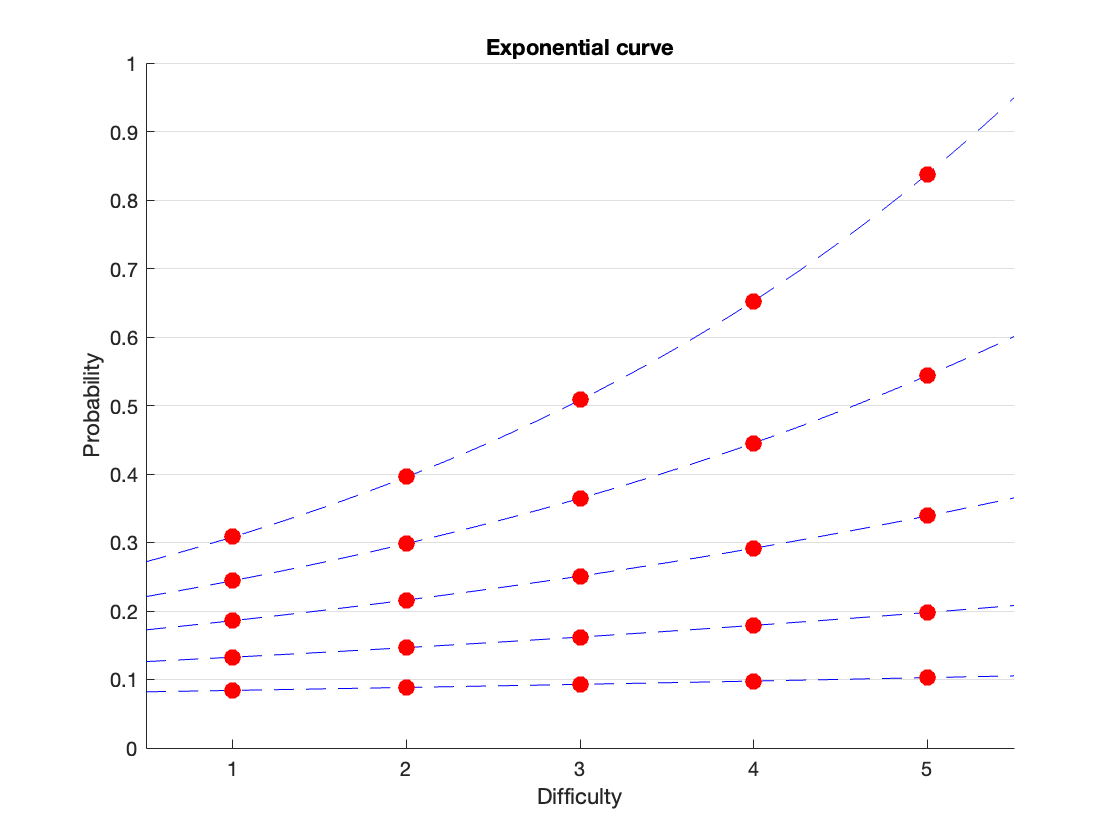
\includegraphics[width=\linewidth]{exp.png}
        \caption{Five possible learning curves following the exponential equation $\vartheta(d) = ae^{b(d-1)}$.}
        \label{exp1}
    \end{subfigure}\hspace{0.05\linewidth}
    \begin{subfigure}[b]{0.4\linewidth}
        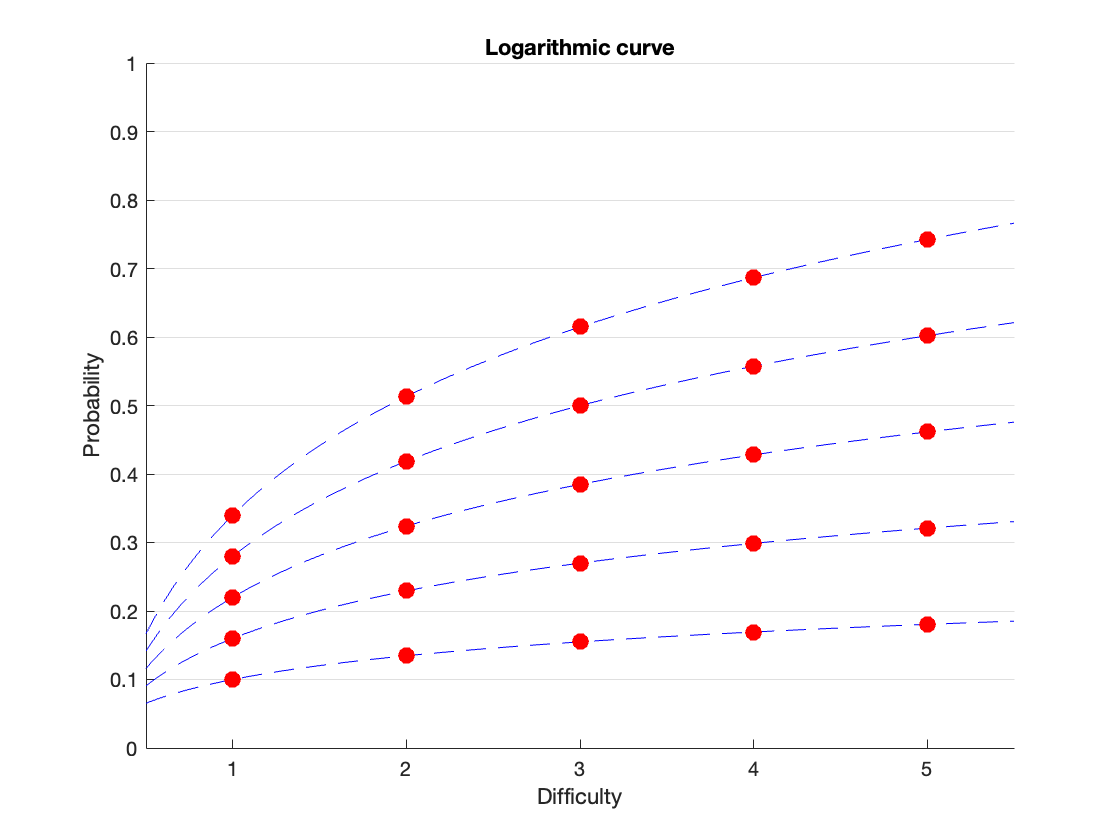
\includegraphics[width=\linewidth]{log.png}
        \caption{Five possible learning curves following the logarithmic equation $\vartheta(d) = a + b\ln d$.}
        \label{log1}
    \end{subfigure}
    \caption{Predictions of the \textsl{exponential} \eqref{exp1} and the \textsl{logarithmic} \eqref{log1} curves.}
    \label{fig1}
\end{figure}

After computing all the learning curves, it is possible to make exponential and logarithmic regressions on those curves, to find the parameters $a$ and $b$.
Then, the residuals are calculated and the regression with smaller residuals gets assigned to the learning curve.
Finnaly, to get two variables within the same range of values, $\openinter{0}{1}$, we retrieve the value $a$ and the value $b'=-\frac{4b}{\ln a}$, for \eqref{eqexp}, or $b'=\frac{b\ln 5}{1-a}$, for \eqref{eqlog}.
\section{Intelligent Tutoring System}
But how will the mixture model schedule practice routines for a student? The current method of SIACUA already uses bayesian networks to create a solid way to estimate a student's progress, but there isn't any approach to formulating schedules.
Furthermore, the beliefs are just used as a prior for the values of the learning curves and are not sufficient to predict whether or not the student has mastered a certain topic.

So, the goal of the ITS it to gather information about the beliefs and the parameters of the regressions in \eqref{fig1} and schedule practice routines for the students, based on suggestions and spontaneous feedback. Moreover, since various topics are taken into account, the algorithm \eqref{alg1} has to be used in another context, to provide more individual results about each student.
\subsection{Variables}
Every time a student answers a question, the ITS should calculate and store a series of variables that will help it deciding what to recommend to the student.
There are two types of variables: \textsl{static variables} and \textsl{topic related variables}. The first ones are:
\begin{itemize}
    \item $T_\mathit{tutor}$ — tendency to follow the ITS' recommendations. Let $t \in \{0,1\}$ be the outcome for a new recommendation that pops up.
    Considering the vector ${\bf t}$ of the outcomes, each $t_i$ is a realization of a random variate $T_i \sim \mathcal{B}(p)$, with $0 < p < 1$, and because the newest values are more significant ($t_0$ is newer than $t_1$), if $X \sim \text{Geo}(p)$, then
    \begin{align*}
        T(p) &= \sum_{i=0}^{n-1} t_i \cdot \mathbb{P}(X = i), \\
        T_\mathit{tutor} &= \max\left\{\left.T(p)\right|_{\frac{\partial}{\partial p}T(p) = 0}\right\}.
    \end{align*}
    It's possible to show that
    \begin{alignat*}{2}
        && 0 &= \frac{\partial}{\partial p}T(p) \\
        \LRA && 0 &= \sum_{i=0}^{n-1} t_i\left(1-(i+2)p\right)(1-p)^i,
    \end{alignat*}
    and after computing the possible values for $p \in \openinter{0}{1}$, they are again plugged in $T(p)$ and the maximum of those values will be the tendency $T_\mathit{tutor}$.
    \item $n_s$ — number of questions answered during the current session. Since this value ranges from $0$ to $+\infty$, it's normally interpreted as a Poisson distribution $N \sim \text{Pois}(\lambda_s)$, where $\lambda_s$ is the average of the number of questions answered each session, that is stored and updated everytime the session ends.
    It is used its cumulative distribution function to calculate the critical value for which the result is greater than $c$:
    \begin{align*}
        \mathbb{P}(N \le n_c) &= \sum_{i=0}^{n_c} \mathbb{P}(N = i), \\
        \mathbb{P}(N \le i-1) < c \le \mathbb{P}(N \le i) &\Rightarrow n_c = i.
    \end{align*}
    \item $t$ — current time spent on a single question, measured in seconds. The ITS will also keep record of the mean value $\mu_t$, the mean of the squares $\mu_{t^2}$ and the sample standard deviation $\sigma_t$, updating it everytime a new value of $t$ is stored:
    \begin{align*}
        \mu'_t &= \frac{n_s\mu_t + t}{n_s + 1} \\
        \mu'_{t^2} &= \frac{n_s\mu_{t^2} + t^2}{n_s + 1} \\
        \sigma_t &= \sqrt{\mu_{t^2} - \mu_t^2}.
    \end{align*}
    This way, since the variate that measures time is $T \sim \mathcal{N}(\mu_t, \sigma^2_t)$,
    $$ Z_t = \frac{T-\mu_t}{\sigma_t} \sim \mathcal{N}(0,1). $$
    To find the critical value from which the cumulative distribution function has values above $c$, we calculate
    \begin{alignat*}{2}
        && \mathbb{P}(Z_t \le z_c) &\ge c \\
        \LRA && \mathbb{P}\left(\frac{T-\mu_t}{\sigma_t} \le z_c\right) &\ge c \\
        \LRA && \mathbb{P}\left(T \le z_c\sigma_t + \mu_t\right) &\ge c \\
        \LRA && z_c\sigma_t + \mu_t &= t_c.
    \end{alignat*}
\end{itemize}
Apart from the first variables, the other \textsl{static variables} are reseted once the current session ends. The \textsl{topic related variables} are:
\begin{itemize} 
    \item $T_\mathit{miss}$ — tendency to make a mistake on a question. The calculations made are the same as the ones for $T_\mathit{tutor}$. Considering the error vector ${\bf e}$ and $X \sim \text{Geo}(p)$, for $0<p<1$,
    \begin{align*}
        T(p) &= \sum_{i=0}^{n-1} e_i \cdot \mathbb{P}(X = i), \\
        T_\mathit{miss} &= \max\left\{\left.T(p)\right|_{\frac{\partial}{\partial p}T(p) = 0}\right\}.
    \end{align*}
    \item $n$ — number of questions answered. Because this variable is relative to each topic, we don't need to assign a certain distribution because it will just define the shape of our later distributions.
    \item $t_q$ — current time spent on a single question, measured in seconds. The same variables as in $t$ are stored and we're left with the distribution
    $$ Z_{t_p} = \frac{T_p-\mu_{t_p}}{\sigma_{t_p}} \sim \mathcal{N}(0,1), $$
    and the critical value is also retrieved with
    \begin{alignat*}{2}
        && \mathbb{P}(Z_{t_p} \le z_c) &\ge c \\
        \LRA && z_c\sigma_{t_p} + \mu_{t_p} &= (t_p)_c.
    \end{alignat*}
    \item $S$ — success rate. It's a ratio between the number of correct answers by the number of questions answered. The \textsl{lazy} value for the variable would be plain division between the number of right answers and $n$, but since time has also an important role on the success rate, a more accurate value would be $(1-p)$, where $p$ is the value assigned when calculating $T_\mathit{miss}$. The critical value for the success $p_c$ is the value that represents stagnation in progress.
    \item $b$ — current belief, retrieved from the bayesian network. This values are already computed by the web application but the ITS stores them for convenience. If we regard $B \sim \Beta{\alpha}{\beta}$ as a \textsl{clumsy} variate that models beliefs, where $\alpha$ and $\beta$ are the number of right and wrong answers, respectively, then as $\alpha$ and $\beta$ grow large,
    \begin{align*}
        B &\overset{a}{\sim} \mathcal{N}\!\left(\frac{\alpha}{\alpha+\beta}, \frac{\alpha\beta}{(\alpha+\beta)^2(\alpha+\beta+1)}\right) \\
        Z_b &= \frac{B - \frac{\alpha}{\alpha + \beta}}{\sqrt{\frac{\alpha\beta}{(\alpha+\beta)^2(\alpha+\beta+1)}}} \sim \mathcal{N}(0,1).
    \end{align*}
    If we assign $\alpha + \beta = n$, then $\alpha \approx nb$ and
    \begin{align*}
        \frac{\alpha}{\alpha+\beta} &\approx \frac{nb}{n} = b, \\
        \frac{\alpha\beta}{(\alpha+\beta)^2(\alpha+\beta+1)} &\approx \frac{nb(n-nb)}{n^2(n+1)} = \frac{b(1-b)}{n+1}.
    \end{align*}
    and with the same calculations with the time variables, the critical value would be
    \begin{alignat*}{2}
        && \mathbb{P}(Z_b \le z_c) &\ge c \\
        \LRA && b + z_c\sqrt{\frac{b(1-b)}{n+1}} &= b_c.
    \end{alignat*}
    \item $b_n$ — average value of the beliefs from a topic and its neighbours. This variable follows the same logic as $b$ for the normal distribution.
\end{itemize}

\subsection{Decisions}
After computing and storing all the variables, the ITS performs addicional calculations to find if it needs to recommend something to the student. 
To accomplish this, it corresponds each study suggestion with a variate such that all variates follow the same kind of distribution.
Since we are dealing with multiple parameters and the ITS should only recommend something after crossing some threshold value, it is used the Generalized Extreme Value distribution for every tip.

In a distribution of the type $A \sim \GEV{\mu}{\sigma}{\xi}$, the first parameter $\mu$ represents the location, the value from which the model starts recognizing that some action shoud be taken.
The second, $\sigma$, it's the scale parameter, turning the curve wider as it gets bigger. The last one, $\xi$, it's the shape parameter, that defines the structure of the tail. On this context, we want only positive values (exceptionally 0, also), noticing that the curve gets more steep near $\mu$ as $\xi$ increases.

The $6$ suggestions are:
\begin{itemize}
    \item \textsl{Learn this topic}. You have little knowledge about it and have answered almost no questions.
    \begin{align*}
        A_\mathit{learn} &\sim \GEV{b_c}{\sqrt{\frac{b(1-b)}{n+1}}}{n} \\
        \mathbb{P}_\mathit{learn} &= \mathbb{P}\left(A_\mathit{learn} \le 1 - b\right)
    \end{align*}
    \item \textsl{Do a quick scan}. You are spending too much time answering these questions and you are answering incorrectly most of the questions.
    \begin{align*}
        A_\mathit{scan} &\sim \GEV{(t_p)_c}{{\sigma_t}_p}{S} \\
        \mathbb{P}_\mathit{scan} &= \mathbb{P}\left(A_\mathit{scan} \le t_p\right)
    \end{align*}
    \item \textsl{Revise these concepts}. You are making too many mistakes and you have little knowledge about that topic and neighbouring topics.
    \begin{align*}
        A_\mathit{revise} &\sim \GEV{(b_n)_c}{\sqrt{\frac{b_n(1-b_n)}{n+1}}}{T_\mathit{miss}} \\
        \mathbb{P}_\mathit{revise} &= \mathbb{P}\left(A_\mathit{revise} \le 1 - b_n\right)
    \end{align*}
    \item \textsl{Deepen this topic}. I see you listen to my recommendations but you still aren't making any progress whatsoever.
    \begin{align*}
        A_\mathit{deepen} &\sim \GEV{p_c}{\sqrt{S(1-S)}}{1-T_\mathit{tutor}} \\
        \mathbb{P}_\mathit{deepen} &= \mathbb{P}\left(A_\mathit{deepen} \le S\right)
    \end{align*}
    \item \textsl{Focus on this topic}. Inspite of answering to a lot of questions about this, you seem to have low knowledge about it.
    \begin{align*}
        A_\mathit{focus} &\sim \GEV{b_c}{\sqrt{S(1-S)}}{\frac{1}{n}} \\
        \mathbb{P}_\mathit{focus} &= \mathbb{P}\left(A_\mathit{focus} \le 1 - b\right)
    \end{align*}
    \item \textsl{Time to take a break}. I see you are spending too much time in every question and you have already answered a lot of questions in this session.
    \begin{align*}
        A_\mathit{break} &\sim \GEV{t_c}{\sigma_t}{\frac{1}{n_s}} \\
        \mathbb{P}_\mathit{break} &= \mathbb{P}\left(A_\mathit{break} \le t\right)
    \end{align*}
\end{itemize}

After calculating all the probabilities, we perform a $t$-test on the maximum probability, where the significance level is determined by the beliefs, because the higher the knowledge level in some topic, the less the need of practice scheduling.
\begin{align*}
    \mathbb{P} &= \left\{\mathbb{P}_\mathit{learn}, \mathbb{P}_\mathit{scan}, \mathbb{P}_\mathit{revise}, \mathbb{P}_\mathit{deepen}, \mathbb{P}_\mathit{focus}, \mathbb{P}_\mathit{break}\right\}, \\
    M_\mathbb{P} &= \max\{\mathbb{P}\}, \\
    \mathbb{P}' &= \mathbb{P}\backslash M_\mathbb{P}, \\
    U &= \overline{\mathbb{P}'} + t_{4,b}\frac{s_{\mathbb{P}'}}{\sqrt{5}}.
\end{align*}
If $M_\mathbb{P} > U$, then we must reject the null hypothesis and conclude that the action associated with $M_\mathbb{P}$ should be recommended, with a significance level of $b$.

\subsection{Tutoring Curves}

The only variable that's missing its calculation is the variable $c$ for the critical value. That's when the tutoring curves take place, using the same algorithm \eqref{alg1}.
However, instead of using data from all students, just the last $10$ tests from the student that will perform the next test are taken into account. We initiate the algorithm with three components:
\begin{enumerate}
    \item a primary component, with random values for $\vartheta_k$, but where the prior for $\alpha_k$ and $\beta_k$ are the ones calculated by the \textsl{clumsy} variate that models the beliefs, using the current belief.
    \item a \textsl{lucky} component, with random values for $\vartheta_k$, $\alpha_k = 0$ and $\beta_k$ is equal to the number of questions answered per test.
    \item an \textsl{unlucky} component, with random values for $\vartheta_k$, $\beta_k = 0$ and $\alpha_k$ is equal to the number of questions answered per test.
\end{enumerate}
By the properties of the algorithm \eqref{alg1}, the \textsl{lucky} and \textsl{unlucky} components model the extreme case where the student could answer all questions right and wrong, respectively, providing curves with very low and very high probabilities.
After answering the questions of the new test, the ITS would then apply the results onto the mixture model to find the curve where the student fits the most, recording the percentage of the likelihood of the primary component (represented by $\mathbb{L}$), relative to the others.
\begin{align*}
    \mathbb{P}({\bf e}) &= \sum_{k \in \left\{\mathit{primary},\mathit{lucky},\mathit{unlucky}\right\}} \rho_k \cdot \varpi\left(\boldsymbol{\mathcal{B}}\left({\bf Q}^T \cdot \boldsymbol{\vartheta}_k, {\bf e}\right)\right) \\
    \mathbb{L} &= \frac{\rho_\mathit{primary} \cdot \varpi\left(\boldsymbol{\mathcal{B}}\left({\bf Q}^T \cdot \boldsymbol{\vartheta}_\mathit{primary}, {\bf e}\right)\right)}{\mathbb{P}({\bf e})}.
\end{align*}
The variable $\mathbb{L}$ measures how consistent the student's practice routines are, so the lower the value, the lower is the confidence that the test is truthful. If the primary tutoring curve is too close to the lucky or unlucky tutoring curves, then we discard the one closest to the primary one.

Then, using exponential or logarithmic regressions, the values for $0<a<1$ and $0<b'<1$ are calculated to get the critical value $c$.
We place the point $(a,b')$ in the rectangle $R = \openinter{0}{1}\times\openinter{0}{1}$ and compute the distance from the point to the corner $(1,1)$.
Although, we need to account for $\mathbb{L}$, as the lower it is, the close to the center of the rectangle the points goes. With a bit of vector algebra,
\begin{alignat*}{2}
    && (x,y) &= \left(a + (1-\mathbb{L})\left(\frac{1}{2} - a\right),b' + (1-\mathbb{L})\left(\frac{1}{2} - b'\right)\right) \\
    \LRA && (x,y) &= \left(\frac{1}{2}+\mathbb{L}\left(a-\frac{1}{2}\right),\frac{1}{2}+\mathbb{L}\left(b'-\frac{1}{2}\right)\right) \\
    \LRA && (x,y) &= \frac{1}{2}\left(1+\mathbb{L}(2a-1),1+\mathbb{L}(2b'-1)\right)
\end{alignat*}
From that, we normalize the distance and
\begin{align*}
    c &= \frac{\left\|(x,y) - (1,1)\right\|}{\sqrt{2}}.
\end{align*}
This means that the lower the distance, the lower the critical value for the threshold for the ITS' recommendations. This can produce very high results to all decision thresholds but since we are performing $t$-tests to ponder which suggestion to make, it just prompts the ITS to schedule practice routines more regularly.

\section{Notifications and Constructing Feedback}
Apart from the 6 main suggestions, the ITS should also be able to provide notifications and constructive (either positive and negative) feedback in real-time. While the notifications are shown before the test, feedback is shown during each test and not at the end, and uses different criteria for possible suggestions.

Evey time a student clicks on a notification or answers a question, the ITS learns something about that student and, based on that information, provides other notifications and feedbacks that enhances his study performance.
We call this the \textsl{reward}, and everytime the ITS is prompted to give notifications and feedback, it calculates the one with the highest reward.

\subsection{Notifications}
Notifications will just pop up on the main page of the web application. They are clickable links that redirect the user to some page or exercise.
Every time the student logs on, the notification with highest reward at the moment will appear. Subsequent visits to the main page will not always produce notifications.
\subsubsection{Reward}
Every notification can be clicked or ignored, and after being clicked it can either result in a success or in a failure.
So, for every notification $t$ we have the set of outcomes $c_t = \{0,1\}$ for the click and $r_t = \{0,1\}$ for the success.

We say a notification is elegible when it meets certain criteria, like test-streaks and belief values.
\subsubsection{List of Notifications}
\begin{itemize}
    \item \textsl{You are missing out on <topic>}.
    \item \textsl{Continue your streak on <topic>}.
    \item \textsl{Have you studied <topic> today?}
    \item \textsl{<Random question about one topic>}.
\end{itemize}
\subsection{Feedback}
\subsubsection{Reward}
\subsubsection{List of Feedbacks}
\begin{itemize}
    \item \textsl{Level Up!} (positive).
    \item \textsl{Level Down...} (negative).
    \item \textsl{Nice streak! Keep it up!} (positive).
    \item \textsl{You missed a few in a row, take your time to answer...} (negative).
    \item \textsl{You're nailing it! Just a few more to go!} (positive)
    \item \textsl{Don't give up, just a few more to go!} (negative)
\end{itemize}
\subsection{Test Layout}
Each test consists on a number $N$ of questions of progressing difficulties. Consecutive right and wrong answers lead to going up or down levels of difficulty, respectively.
After each question, the ITS computes the feedback with highest reward and provides it. The 

\section{Programming}
Since SIACUA is programmed in C$\sharp$, the ITS will also be constructed in that language, as a Class Library (.dll file), to be then used as a reference for this and other web applications.

\end{document}